% !TeX root = ../thuthesis-example.tex

\chapter{绪论}
自然界中存在大量复杂的拓扑结构,例如衍架结构和蜂窝状结构。这些复杂拓扑结构不仅在力学性能方面表现出优异的性价比,而且在生物学层面也展现出有利于细胞生长繁衍的亲和性。因此,这类复杂拓扑结构在轻量化设计和人造生物体植入等领域得到广泛应用。
得益于3D打印技术的快速发展和普及,制造和生产这些复杂拓扑结构已不再是问题。工程力学、生物学和材料学等领域的专家设计出了越来越多结构多样化、功能丰富的复杂拓扑结构。近几年,随着计算机技术的发展,拓扑优化方法成为复杂结构设计和优化的主要工具。

拓扑优化是一种基于材料分布优化的结构设计方法,在满足性能需求的前提下,可最大限度地减少材料使用成本。这一研究方向符合我国绿色、可持续发展的理念,也是促进智能制造技术发展的关键所在。
拓扑优化可应用于各类结构的最优化设计,以实现强度、热传导效率、制造性能等目标需求。一般而言,拓扑优化主要包括结构表示、仿真分析和优化求解三个关键环节。然而,复杂结构的表示、分析和优化求解效率往往较低,严重制约了拓扑优化技术在工程实践中的应用。
因此,进一步深入研究针对不同目标的拓扑优化理论,开发更加高效、鲁棒的算法,对于促进智能制造技术的发展至关重要。本研究的核心在于从结构表示入手,利用结构的隐式表示,探索提高面向不同应用需求的结构优化算法效率和稳定性的方法。

\section{拓扑优化}
拓扑优化理论的发展已有三四十年历史。由于地球资源有限,如何高效、经济地利用能源和原材料,一直是人类追求的目标。拓扑和结构优化正是解决这一问题的关键,其目的是以最少的材料和最低的消耗,达到结构的目标性能,包括强度、刚度、稳定性和散热等。
将优化方法应用于结构设计,不仅可大幅缩短设计周期,显著提高设计质量,还可解决传统设计方法无法解决的复杂问题。总的来说,结构优化即在给定约束条件下,寻找目标函数的极值。在拓扑优化中,目标函数可以是结构的刚度、体积、变形、自振频率、振幅等。
随着3D打印技术的发展,拓扑优化作为一种结构设计方法,也被广泛应用于增材制造的前端设计,如支撑结构优化、内部填充结构生成等。下面将介绍总结几种主流的结构拓扑优化方法。
\begin{figure}[htbp]
    \centering
    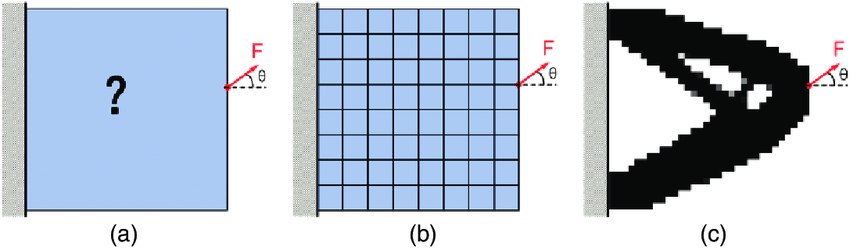
\includegraphics[width=1.0\linewidth]{./figures/intro-simp}
    \caption{2D SIMP拓扑优化方法示意图~\cite{luo_simp2021}}
    \label{fig:simp}
\end{figure}
\subsection{匀质化方法}
均匀化理论是一种确定等效均匀化材料属性的方法。1988年,Bendsoe和Kikuchi提出了首个连续体结构拓扑优化的均匀化方法\cite{BENDSOE1988}。该方法将宏观结构划分为单元胞,以单元胞结构属性(如材料密度、弹性模量、几何尺寸等)作为设计变量,将拓扑优化问题转化为单元胞微结构尺寸优化问题。随后,他们又提出了二维和三维结构的均匀化方法\cite{GUEDES1990}。
Michel等人利用均匀化方法研究了复合材料周期微结构的计算方法\cite{MICHEL1999}。吴长春等人采用均匀化方法优化了复合材料的极值弹性特性和最大刚度,实现了微结构的拓扑优化设计\cite{Yuan2003}。谢天海等人利用均匀化方法对柔顺结构进行了拓扑优化研究\cite{Xie2003}。王晓明等采用均匀化理论和伴随变量法分析了连续体结构拓扑优化的灵敏度,表现出良好的数值计算性能\cite{Wang1999}。
需要注意的是,由于均匀化方法存在构造微结构和设计变量过多等问题,其主要应用于材料微观设计领域。
\subsection{SIMP方法}
变密度法是在均匀化方法基础上发展而来。该方法将设计域离散为有限单元网格,以每个单元或节点的相对密度作为设计变量,利用密度惩罚方法使相对密度在1和0之间连续变化。
SIMP方法(实体各向同性材料惩罚模型)是一种基于变密度法的拓扑优化方法,如图~\ref{fig:simp}所示,展示了SIMP拓扑优化方法的一个2D示例。SIMP方法最早由Rozvany等人提出\cite{Rozvany1992}。他们验证了SIMP方法的最终优化结构与采用均匀化方法得到的结果一致。Sigmund和Bendsoe探索了多种变密度法材料插值模型\cite{Bendsoe2003,Bendsoe1999},指出SIMP方法中产生的中间密度值具有物理意义,并验证了指数形式的材料插值模型具有广泛适应性。Rozvany等人详细介绍了SIMP方法的起源、理论背景及主要优缺点\cite{Rozvany2001}。
Yuan等人在变密度法中成功引入了杂交单元,实验结果表明可获得更优的拓扑优化结果,并克服了棋盘格现象\cite{Yuan2001}。李翔等人提出过滤函数方法来解决SIMP方法中灰度单元过多的问题。Martinez等人研究了SIMP方法的收敛性,给出了更弱的假设条件\cite{Martinez2005}。
变密度法具有较强的普适性,适用于各类拓扑优化问题,因此在连续体结构拓扑优化中应用广泛。


\subsection{水平集方法}
水平集方法最早主要应用于图像处理和流体力学中的运动边界跟踪,由Sethian和Osher等人提出~\cite{OSHER1988,OSHER2001}。如图~\ref{level-set}所示,其主要思想是将移动边界作为零水平集嵌入高维水平集标量函数中,这样就可以利用闭曲面演化的方法得到水平集函数的演化方程,而嵌入的闭曲面总是其零水平集,最终只需确定零水平集即可确定移动界面的演化结果。
水平集方法具有几何直观性强、能够处理拓扑变化等优点,因此在结构优化领域也得到广泛应用。2000年,Sethian等人将水平集方法成功应用于结构优化~\cite{SETHIAN2000}。Wang等人利用方向导数进行灵敏度分析,将水平集方法应用于均匀材料、多材料、柔性机构的拓扑优化设计~\cite{Wang2003,Wang2004}。庄春刚等人比较了水平集方法与SIMP方法,指出水平集方法得到的优化结果具有光滑的几何边界,数值算法更稳定~\cite{zhuang2007}。
此外,水平集方法还被应用于结构形状优化、多目标优化、动态优化等领域。
\begin{figure}[htpb]
\centering
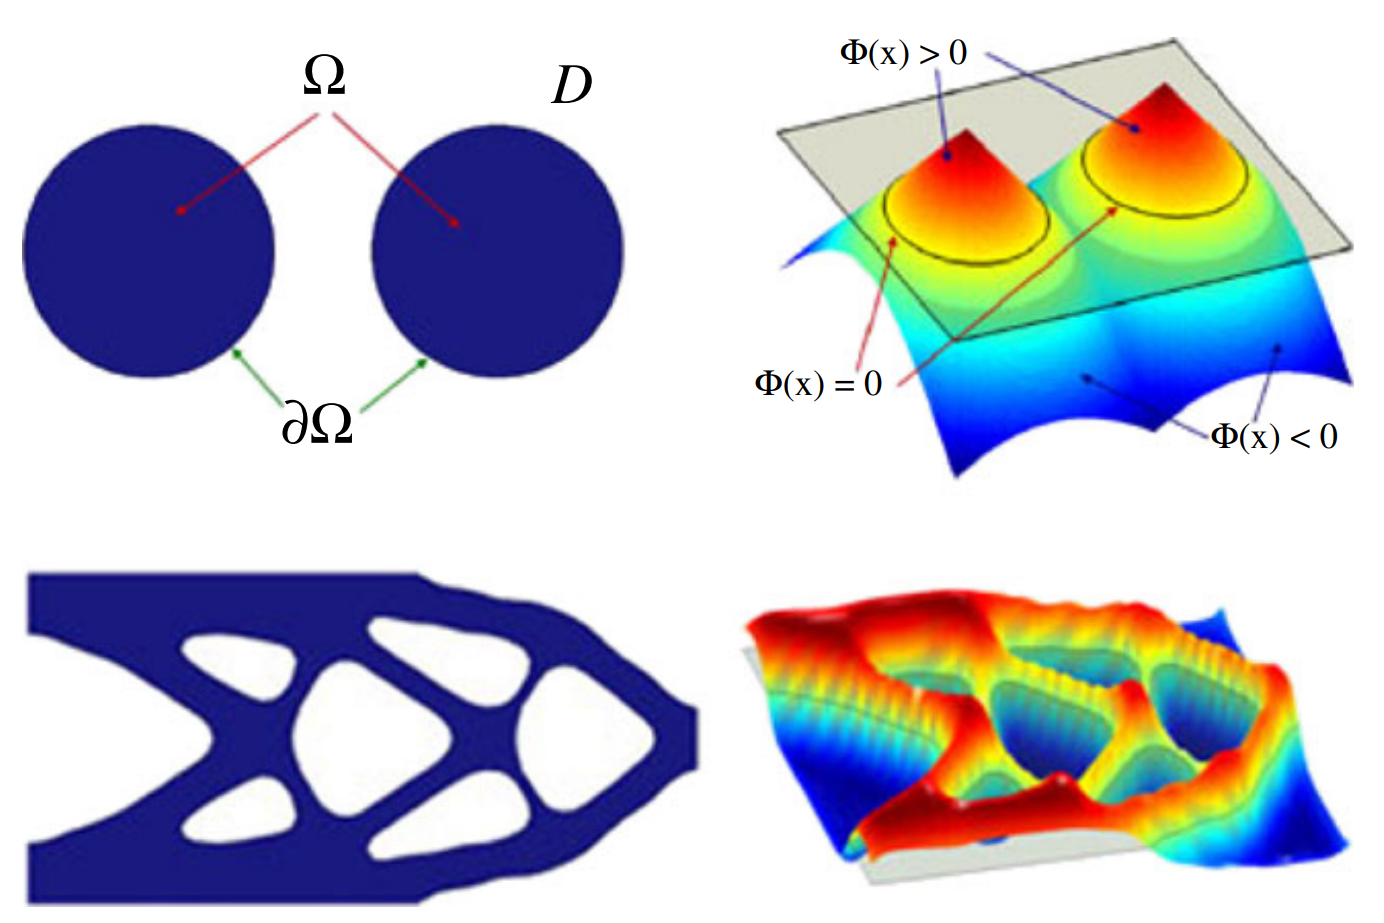
\includegraphics[width=0.9\linewidth]{./figures/intro-level}
\caption{水平集方法~\cite{deaton2014survey}}
\label{level-set}
\end{figure}

\subsection{MMC/MMV方法}
从几何表示的角度来看,以上方法都是在基于像素或节点的求解框架内开发的。这些方法虽然取得了显著的成果,但仍存在一些具有挑战性的问题需要进一步解决:
首先,基于像素的拓扑表示与现代计算机辅助设计(CAD)建模系统并不完全一致,因此无法直接在CAD平台上进行优化。其次,由于基于像素的拓扑优化方法没有明确嵌入几何信息,很难对结构特征尺寸进行精确控制,而在制造方面,这一点通常很重要。最后,采用单元材料分布来表示结构拓扑,基于像素的拓扑优化方法所涉及的计算工作量相对较大,特别是在三维问题中,所需的计算量大得难以想象。水平集方法是基于节点的拓扑优化方法的代表。在水平集方法中,也需要将设计域离散为有限元来计算结构响应,但通常以节点处的水平集函数值作为拓扑设计变量。虽然几何信息(如外法向量和曲率边界等)可以从水平集函数计算,但水平集方法在CAD建模系统中采用的隐式几何表示方式与显式几何表示方式有很大不同,因此基本上具有与变密度法相同的缺点,也无法摆脱维度魔咒。
\begin{figure}[htpb]
\centering
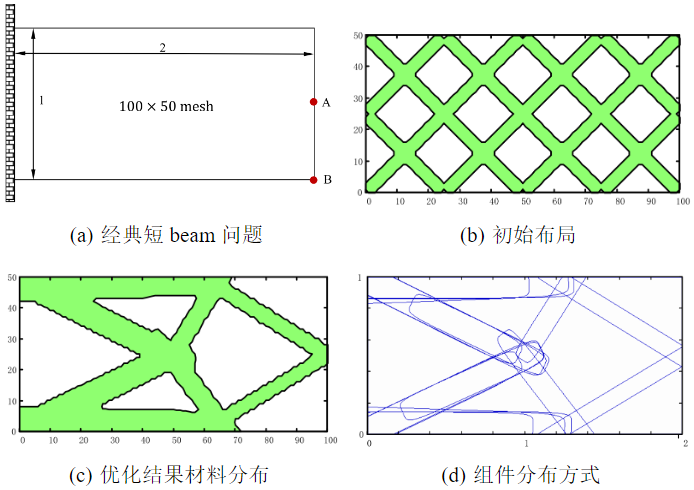
\includegraphics[width=1.0\linewidth]{./figures/intro-mmc}
\caption{可移动变形组件方法~\cite{Zhang2014}(MMC)}
\label{MMC}
\end{figure}
\begin{figure}[htpb]
\centering
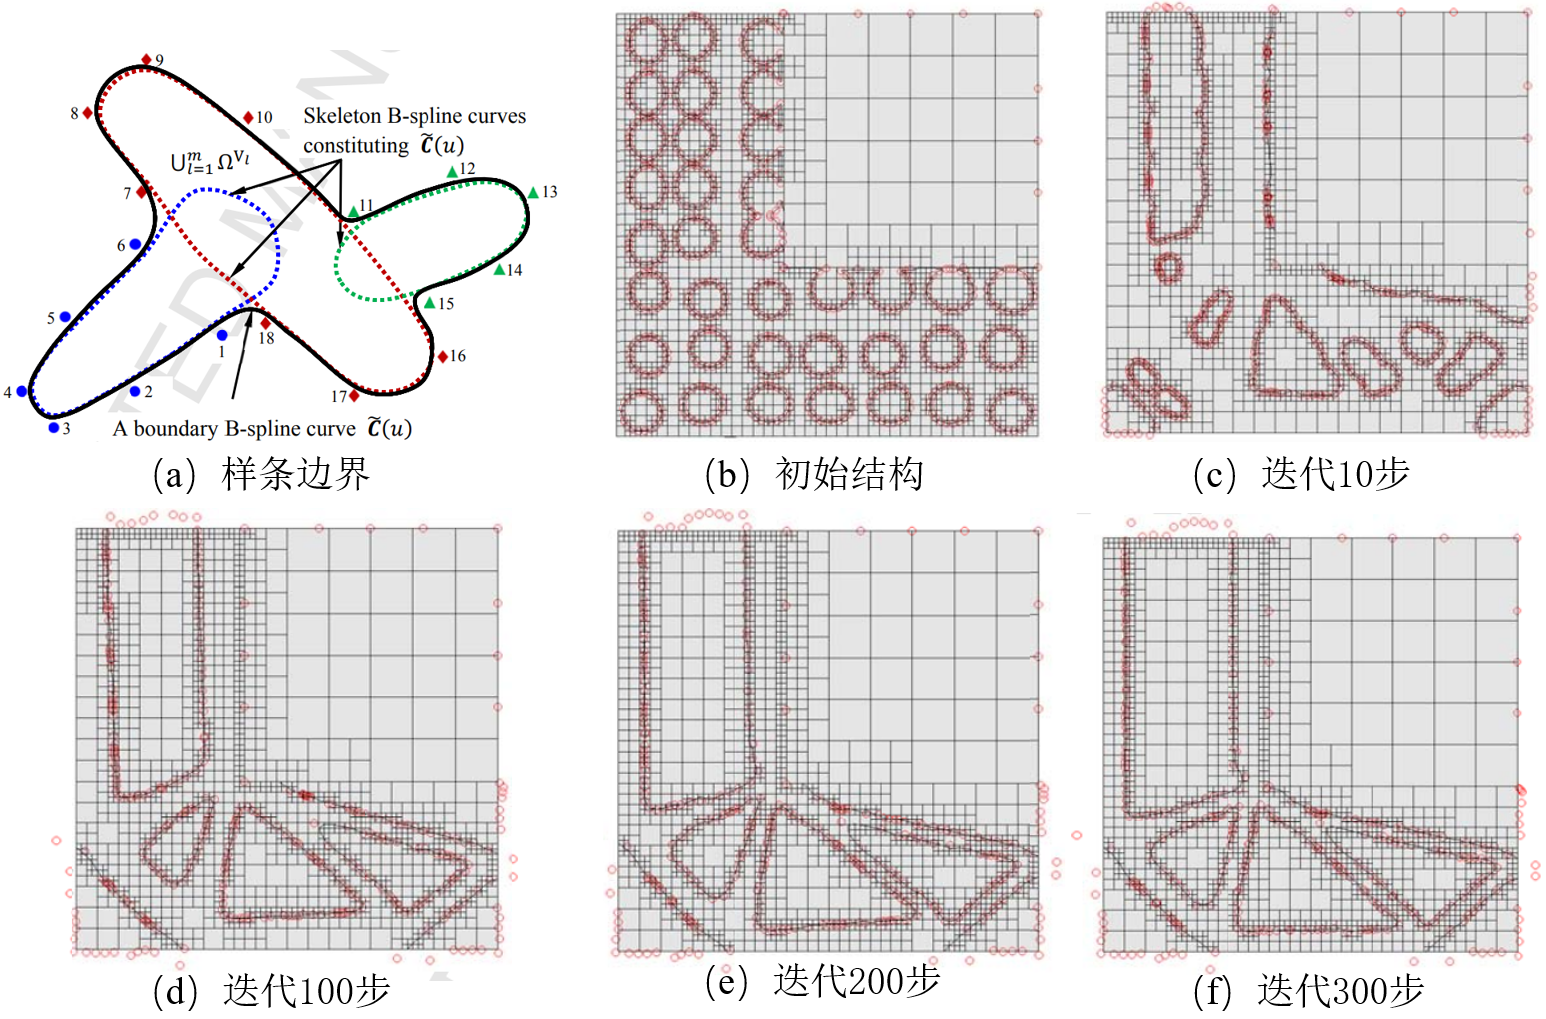
\includegraphics[width=1.0\linewidth]{./figures/intro-mmv}
\caption{可移动变形孔洞方法~\cite{zhang2018moving}(MMV)}
\label{MMV}
\end{figure}
为了建立结构拓扑优化和CAD建模系统之间的直接联系,Guo等人提出了一种更几何化、更灵活的显式化方法——可移动变形组件方法(MMC)~\cite{Zhang2014}。该方法的显著特点是使用一组可变组件作为拓扑优化的构建块,通过优化这些组件的形状、长度、厚度、方向和布局(连通性)来找到最优的结构拓扑。如图~\ref{MMC}所示,对于经典的短梁问题,在A点受竖直向下的力,先在设计域中给定初始的组件分布,然后通过优化得到最终的拓扑优化结构,图~\ref{MMC}(d)显示的就是最终组件的分布方式,由此决定了优化结构的布局。随后,Zhang等人又提出了对偶的可移动变形孔洞方法,如图~\ref{MMV}所示。该方法用样条来确定孔洞的边界,然后通过优化多个样条参数来获取设计域上挖洞区域的确定,从而达到结构优化的目的。

MMC/MMV这种显式方法的一大优点是可以将CAD建模系统的尺寸、形状和拓扑优化无缝地集成在一起,这在工程应用中具有很大潜力。此外,与SIMP、水平集方法相比,它拥有较少的优化变量,在计算上表现出较高的效率和鲁棒性。


\section{结构表示}
结合以上拓扑优化算法的现状分析可以看出,结构的表示方式一定程度上决定了拓扑优化方法的特点和性能,比如SIMP方法中的结构是基于单元密度表示的离散方法,而水平集方法中的结构是基于水平集函数表示的 连续方法。表示方法不同,拓扑优化的优化参数不同。在计算机图形学中,三维几何体通常用网格、样条、点云等方法来表达~\cite{agoston2005computer},这些方法用三角网格、三维点或者样条曲线曲面等基本元来描述几何体的边界,被称为显式表示。与之相区别的是隐式表示,其通过定义一个三维空间中的隐式场函数来表示几何体。
\begin{figure}[htbp]
    \centering
    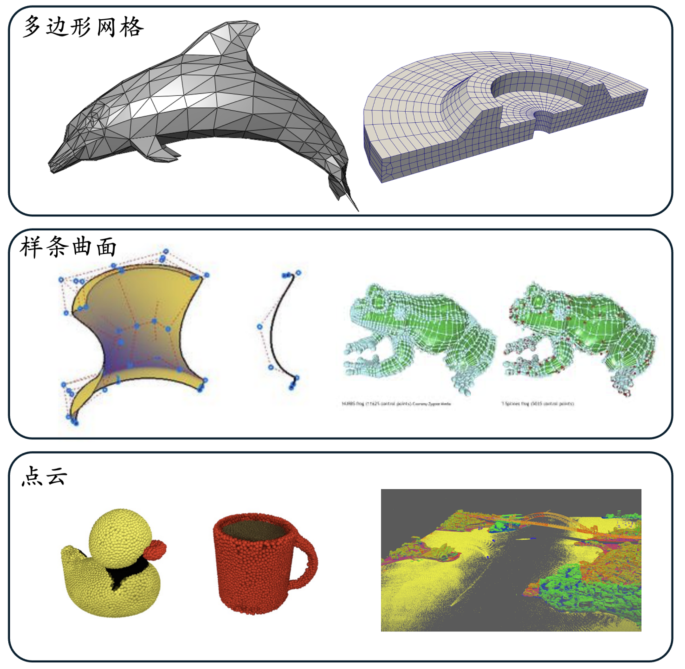
\includegraphics[width=0.48\linewidth]{./figures/intro-explicit-rep}\hfill
    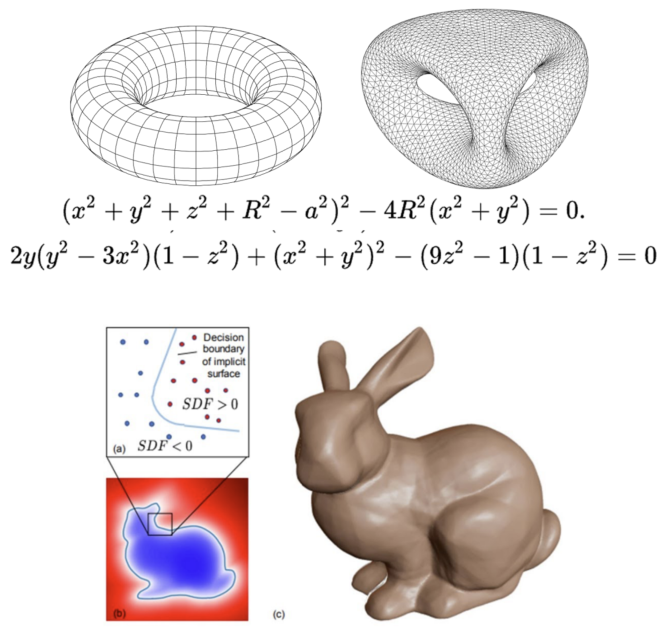
\includegraphics[width=0.48\linewidth]{./figures/intro-implicit-rep}
    \\
    \makebox[0.48\linewidth]{(a)显式表示}
    \hfill
    \makebox[0.48\linewidth]{(b)隐式表示}
    \caption{三维结构的不同表示方法}
    \label{fig:structure-rep}
\end{figure}
\subsection{显式表示}
多边形网格表示是描述三维几何方法中最常用的一种方式,尤其是三角网格表示,如图~\ref{fig:structure-rep} 所示。网格表示的基本元素包括顶点、边和面,这种表示的优点是比较直观,可以表示任意复杂的几何形状,能够通过局部增加顶点和面来精确地描述物体的形状和细节。计算机图形学中也有很多成熟的网格处理算法~\cite{botsch2010polygon},用于几何的表示、变形和布尔等操作。
但是复杂的几何形状需要大量的顶点、边和面等元素信息,导致数据量增大,而且网格表示难以处理具有复杂几何和拓扑特征的几何操作。

在计算机辅助设计(CAD)中,样条表示是一种常用的方法,其通过一组控制点定义的光滑曲线或曲面,能够精确地表示自由形状,常用的有B\'ezier曲线,B-样条和NURBS样条等~\cite{eck1996automatic,熊运阳2014cad},随后发展起来的T-样条克服了传统NURBS样条的局限性~\cite{sederberg2003t,李新2008t},进一步提高了建模的灵活性和效率。样条表示在几何建模中具有显著的优点,包括生成高质量的曲线和曲面、提供灵活的局部控制能力以及能够精确表示形状。然而,其计算和实现的复杂性较高,特别是在处理非光滑特征和局部修改时可能引发全局变化。此外,样条在不同CAD系统之间的兼容性也往往会发生问题。

点云是另一种被广泛应用的三维几何表示方法,其由存在于几何表面的点集合构成~\cite{杨必胜,ran2022surface},除了存储点坐标信息之外,有时还包含其他属性如颜色、法向量等。点云通常通过三维扫描仪、激光雷达等设备获取。点云表示作为一种几何表示方法,具有数据获取便捷、精确度高、灵活性强以及能够直接表示三维空间等优点,但同时也存在数据量大、缺乏拓扑信息、噪声敏感和处理复杂等缺点。这种表示方式在三维重建、自动驾驶~\cite{cui2021deep}、虚拟现实和机器人导航等领域具有广泛应用,尽管面临一定的技术挑战。

\subsection{隐式表示}
几何的隐式表示是一种通过数学函数来描述几何形状的方法。与显式表示不同,隐式表示不直接存储几何体的顶点和边等确定边界的信息,而是通过一个函数来定义几何体的形状。常见的隐式表示包括隐式曲面,距离场(SDF)~\cite{park2019deepsdf,yang2021geometry}和占用率场(Occupancy Field)~\cite{mescheder2019occupancy}等,如图~\ref{fig:structure-rep} (b) 所示。隐式表示使用一个标量函数$f(\mathbf{r})=s$来定义几何体,其中$\mathbf{r}=(x,y,z)\in\mathbb{R}^3$是空间中的坐标。具体来说,对于占用率场,其定义为,
\begin{equation}
f(\mathbf{r})=
    \begin{cases}
        0, & \text{如果}\mathbf{r}\text{是在几何体外部},\\
        1, & \text{如果}\mathbf{r}\text{是在几何体内部}.
    \end{cases}
\end{equation}
而对于有向距离场,其定义为,
\begin{equation}
f(\mathbf{r})
    \begin{cases}
        >0, & \text{如果}\mathbf{r}\text{是在几何体外部},\\
        =0, & \text{如果}\mathbf{r}\text{是在几何体边界},\\
        <0, & \text{如果}\mathbf{r}\text{是在几何体内部},\\
    \end{cases}
\end{equation}
其值代表空间坐标$\mathbf{r}$到几何体表面的最短距离,并通过符号区分几何体的内部和外部。隐式表示通常只需要一个函数即可描述复杂的几何形状,比显式表示更为紧凑,而且几何体之间的布尔运算可通过简单的函数操作即可实现,但是隐式表示的几何体描述不如显式表示直观,理解和操作较为困难。

总的来说,几何的隐式表示是一种强大且灵活的几何描述方法,适用于描述具有复杂形状和拓扑的几何体,但其求解和存储的复杂性也对计算资源和算法提出了较高的要求。

\subsection{隐式神经表示}

\section{基于深度学习的拓扑优化方法}
\begin{figure}[htbp]
    \centering
    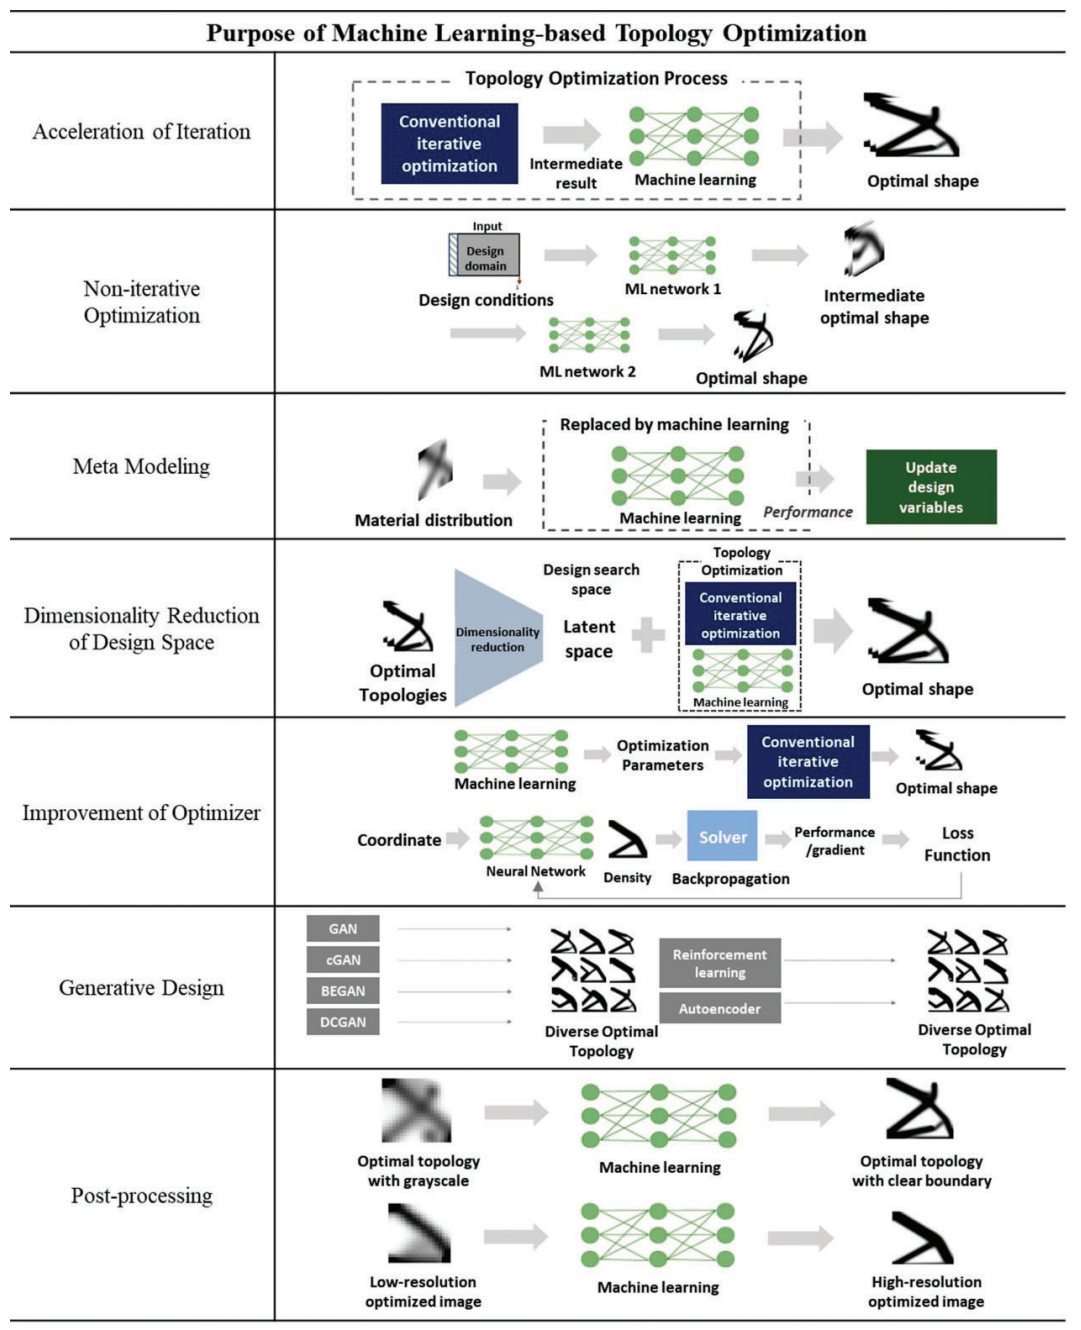
\includegraphics[width=1.0\linewidth]{figures/TOwDL.png}
    \caption{拓扑优化使用学习方法的常见途径~\cite{shin2023topology}}
    \label{fig:TOwDL}
\end{figure}
虽然拓扑优化被认为是一种有效的逆向设计方法,但它面临的一个关键挑战是有限元分析所需的高计算成本;每次迭代优化都必须计算敏感度信息以指导参数调整。对于精细结构的优化,网格分辨率的提高也会导致分析时间显著增长,特别是在解决实际三维问题时,这一挑战尤为突出。因此,众多研究致力于提高拓扑优化的效率,其中神经网络驱动的设计优化方法近年来受到了广泛关注,成为了一个有效的解决途径。如图~\ref{fig:TOwDL} 所示,学习方法目前被用于拓扑优化中用来加速或者改善解的最优性等。
基于神经网络的方法通过其非线性建模能力,将复杂的高维结构优化问题转化为神经网络的参数优化问题,利用梯度反向传播算法和数值优化技术实现结构的快速设计。神经网络加速的拓扑优化方法主要分为两类:

第一类采用端到端的方式,在既定目标和约束条件下直接预测最优化结构,以非迭代的策略实现效率的显著提升。大部分方法将基于密度表示的结构看作二维或三维张量,并利用卷积神经网络(CNN)提取特征,接着通过变分自动编码器(VAE)或者对抗生成模型(GAN)学习结构的特征分布,最后在条件设定下利用学习到的分布直接生成最优结构。最近,在文本图像生成领域取得巨大成功应用的扩散模型(DDPM)也被扩展到端到端拓扑优化算法研究中,大幅提升了准确性和优化效率。

第二类提高效率的方法是利用神经网络替代传统迭代优化过程中耗时的有限元计算和敏感度分析。物理信息神经网络(PINN)是最近备受关注的新兴技术,它通过将物理定律直接嵌入到网络训练中,可以有效地模拟复杂系统的行为,从而规避了传统有限元方法中网格剖分和迭代求解步骤。许多研究已经将 PINN技术与拓扑优化方法相结合,用以替代传统有限元计算,从而提升优化过程的效率。Lee等人通过训练两个独立的 CNN 网络来预测结构的柔度和体积分数,并采用最优性标准(OC)方法更新设计参数。受到图像处理中超分辨率技术的启发,另一种方法利用神经网络从粗精度下的优化结构预测高精度的最优结构,这种方法通过减少维度显著提升了拓扑优化的计算效率。

近期,研究人员已经开始探索利用神经网络技术来设计和优化多孔结构。Kim 等人开发的 ZeoGAN 模型训练了三个神经网络以预测组合数据,成功模拟出真实沸石材料的微孔结构。Kumer 等人采用两个多层感知机(MLP)逆向设计出非周期性的旋转对称细胞结构,并对多孔结构的参数和刚度进行了交叉验证。此外,一些研究利用 VAE 和 GAN 等生成模型实现从图片中重建出多孔结构。Zhang 等人提出了一种整合 VAE 和 GAN的混合模型,提高了从图片生成三维多孔结构的稳定性,并通过引入孔隙损失来提高重建的准确性。超材料是多孔结构的直接应用之一,最近也有许多工作利用神经网络进行超材料单元结构的逆向设计。Wang 等人采用数据驱动的方式,在超材料数据库上训练VAE 模型及用于属性预测的回归器,将复杂的微观结构映射到低维度的连续隐藏空间中,通过简单的空间插值和遍历就可以生成丰富的新型超材料单元孔洞结构。IHGAN结合了GAN生成模型和传统均质化技术,创造出多样化的单元结构,相对于传统密度单一型结构显著提高了超材料结构的性能。然而,现有的神经网络驱动多孔结构设计方法很难与仿真和优化模块整合,这一步骤对于得到满足理想属性的多孔结构并将其应用到实践中至关重要。

\section{本文研究思路及目标}